\subsection{Инерционные колебания. Теорема Тейлора-Праудмена. Сохранение потенциального вихря.}
Инерционные колебания -- колебания, которые обусловлены инерционными силами (центробежной силой, силой Кориолиса).

Величина $\text{П}=(\vec{\xi}+2\vec{\Omega})\cdot\vec{\nabla}\rho$\footnote{$2\vec{\Omega}=\left[\vec{\nabla}\times\left[\vec{\Omega}\times\vec{r}\right]\right]$ -- планетарная завихренность.} называется потенциальным вихрем.
Закон сохранения потенциального вихря (теорема Эртеля):
\begin{equation}\label{eq-3-6-1}
\frac{d\text{П}}{dt}=0
\end{equation}
Для уравнений мелкой воды имеем потенциальный вихрь Россби-Обухова \cite{Должанский-2006}:
\begin{equation}
\text{П}=\frac{\xi+f}{H}
\end{equation}
где $\xi=\vec{k}\cdot\vec{\xi}=\frac{\partial v}{\partial x}-\frac{\partial u}{\partial y}$ -- компонента вдоль оси $z$ относительной завихренности $\vec{\xi}$.
В более общей формулировке потенциальный вихрь называется потенциальным вихрем Эртеля:
\begin{equation}
\text{П}=-g(\xi+f)\frac{\partial\theta}{\partial p}
\end{equation}
где $\theta$ -- потенциальная температура.

\begin{theorem*}[Тейлора-Праудмена]
Стационарные течения во вращающейся идеальной жидкости организованы в серию цилиндров, параллельных оси вращения \normalfont\cite{Гольдштейн-Городцов-2000}.
\begin{equation}
\left(\vec{\Omega}\cdot\vec{\nabla}\right)\vec{v}=0\Rightarrow\vec{v}=\vec{v}(x, y)
\end{equation}
\end{theorem*}
Таким образом, обтекание трёхмерного тела является двумерным (плоским) и совпадает с обтеканием цилиндра, образующие которого параллельны оси вращения и касаются поверхности тела.
Этот цилиндр называется столбом Тейлора (см. рис. \ref{fig:stolb_teilora}).

\begin{figure}[!ht]
\centering
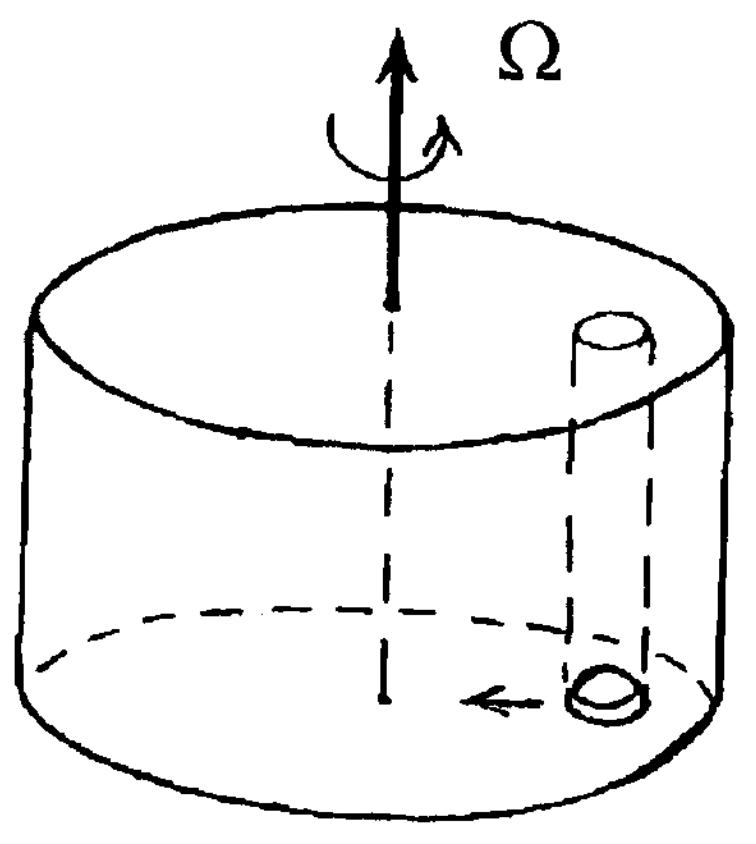
\includegraphics[width=0.25\textwidth]{images/stolb_teilora.png}
\caption{Образование столба Тейлора над медленно горизонтально движущимся телом в быстро вращающейся жидкости \cite{Гольдштейн-Городцов-2000}.}\label{fig:stolb_teilora}
\end{figure}
